\documentclass[journal,twoside]{JoPhA}
\usepackage[utf8]{inputenc}
\usepackage{flushend}
\usepackage{graphicx}
\usepackage{array} 


\begin{document}

\title{Predicción de la mortalidad en accidentes de tráfico}
 
\author{Samuel Rey y David Moreno
\IEEEcompsocitemizethanks{\IEEEcompsocthanksitem Samuel Rey y David Moreno - Universidad Rey Juan Carlos\protect\\

E-mail: samuel.rey.escudero@gmail.com, dmorenolumb@gmail.com.es
%\IEEEcompsocthanksitem Vicente Matell\'an is with University of Rey Juan Carlos.
} % <-this % s
}


\maketitle


\begin{abstract}
Los accidentes de tráfico conllevan un gran coste económico y, sobre todo, humano, por lo que existe un gran interés en ser capaces de predecirlos para, en última instancia, poder evitarlos. Aunque esto supone un gran reto, las técnicas de análisis de datos y aprendizaje máquina ofrecen una oportunidad única para comprender las razones subyacentes que originan estos accidentes. En este artículo utilizaremos estas técnicas para clasificar los accidentes en graves o leves, con el objetivo de predecir la gravedad de los accidentes basándonos en algunas de sus características. De esta forma, sabiendo que determina que un accidente pase de ser considerado leve a ser grave, se podrán tomar medidas para reducir la gravedad y, por lo tanto, la mortalidad de los accidentes. Para conseguir esto hemos realizado un análisis de los datos, hemos comparado distintos modelos y escogido el más adecuado, lo hemos entrenado y evaluado, explicando con detalle cada uno de estos procedimientos y exponiendo las conclusiones principales a las que hemos llegado.
\end{abstract}


%%%%%%%%%% INTRODUCCIÓN %%%%%%%%%%
\section{Introducción}
\IEEEPARstart{L}a predicción de los accidentes de tráfico es uno de los mayores retos de la actual sociedad debido al alto coste económico y, sobre todo, humano que conllevan. Las técnicas de análisis de datos y aprendizaje máquina (\textit{Machine Learning}) ofrecen una oportunidad única para analizar y comprender las razones subyacentes que provocan estos accidentes, otorgando la oportunidad de, en última instancia, predecirlos. En este contexto, los datos recopilados de accidentes anteriores permiten analizar en detalle los factores involucrados para buscar tendencias o patrones. Sin embargo, existen diversos factores que hacen que el análisis de los datos y su utilización para futuras predicciones sea un verdadero reto: \\
	
\begin{itemize}
	\item Las bases de datos son muy grandes y heterogéneas, por lo que habitualmente no se puede o resulta muy complicado trabajar con datos de distintas procedencias. \\
		
	\item Los datos son introducidos manualmente por personas, por lo que son propensos a errores o valores inadecuados y a presentar ruido. Este tema se trata en mayor profundidad en el artículo  \cite{analisis_datos}. \\
		
	\item Las situaciones reales son complejas y sus datos cuentan con un gran número de atributos, por lo que habitualmente consisten en problemas de una gran dimensionalidad, requiriendo un gran número de observaciones para poder resolverlos. \\
		
	\item Las funciones de coste también suelen ser complejas y altamente no lineales, por lo que es sencillo que el algoritmo de optimización se detenga en un mínimo local. Esto además de evitar alcanzar la solución óptima, ocasiona que el resultado del entrenamiento del modelo dependa en gran medida del punto en el que se inicialicen los pesos al comenzar el entrenamiento. \\
\end{itemize}
	
	% Quitar??
	%La utilidad y a la vez, dificultad que esta situación presenta, así como la actual relevancia que está adquiriendo el campo de análisis de datos y aprendizaje máquina, ha motivado la realización de un datatón y concurso en la universidad Rey Juan Carlos. En este datatón se proporcionarán conocimientos básicos en estas materias así como distintos consejos para abordar el problema, haciendo un ranking de las distintas soluciones obtenidas y premiando las dos primeras. \\
	
En este artículo, para abordar este problema nos centraremos en predecir la gravedad del accidente, abordándolo como un problema de clasificación binaria. Basándonos en los atributos \emph{número de heridos leves}, \emph{número de heridos graves} y \emph{número de muertos}, las clases que hemos definido son: \\
	
\begin{itemize}
	\item \textit{Clase 0 - Accidente leve}: consideraremos accidentes leves todos aquellos en los que no haya habido ni muertos ni heridos. \\
	\item \textit{Clase 1 - Accidente grave}: clasificaremos como accidentes graves aquellos en los que haya habido muertos o heridos, ya sean leves o graves. \\
\end{itemize}
	
	
El problema propuesto en este artículo pertenece a un concurso denominado \emph{DATATÓN URJC 2017}, que consiste en una competición de \textit{Machine Learning} con datos reales en el que los participantes pueden formar equipos para crear un modelo y competir para conseguir la mejor puntuación sobre el conjunto de test, seleccionado por los organizadores de este evento. Por lo tanto, esta definición de clases ha sido establecida en las bases de este el concurso, y la máquina explicada en este artículo ha sido ha sido propuesta como solución. Esto supone una dificultad añadida, dado que el conjunto de test utilizado para evaluar las diferentes máquinas presentadas tenía las clases desbalanceadas. Aproximadamente el 75\% de elementos del conjunto de test pertenecen a la clase 1, mientras que sólo el 25\% restante representa a la clase 0. Sin embargo, el conjunto de datos de entrenamiento no estaba desbalanceado. En él, el 54\% de las observaciones pertenecían a la clase 1 y el otro 46\% a la clase 0. \\
	
La base de datos utilizada consta de más de 9000 observaciones, con 83 atributos cada una. Se trata de datos muy ruidosos y de una dimensionalidad elevada, algo que resulta especialmente problemático, como se explica en detalle en \cite{alta_dimensionalidad}. Además, la mayoría de los atributos son paramétricos, por lo que presenta pocos \textit{outliers}. Sin embargo, algunos atributos presentan un gran número de elementos incorrectos. Todo esto hace que sea necesario una primera fase de procesamiento de datos y selección de características antes de elegir y entrenar el modelo, para tener en cuenta sólo las características que realmente aportan información y ayudan a mejorar el rendimiento de la máquina. Esta fase de análisis de datos es especialmente importante, dado que ayuda a evitar sobreaujustes y que el modelo aprenda errores existentes en los datos, o incluso el propio ruido. Cómo se comenta en \cite{extraccion_datos}, un buen análisis previo ayuda a evitar el sobreajuste favoreciendo la generalización, y puede conseguir que un modelo sencillo supere el rendimiento de modelos mucho más complejos. \\
	
A continuación, se explicará detalladamente la metodología empleada para resolver el problema. Se comentará en que ha consistido el análisis de datos realizado, los distintos modelos que se han considerado para resolver el problema y las figuras de mérito que hemos evaluado. Después, detallaremos los dos modelos con los que hemos obtenido un mejor resultado comentando los parámetros de cada uno, y para finalizar, expondremos las conclusiones a las que hemos llegado después de enfrentarnos a este problema. \\

%%%%%%%%%% METODOLOGÍA %%%%%%%%%%
\section{Metodología}
\IEEEPARstart{P}ara enfrentarnos al problema lo hemos dividido en dos fases distintas. En primer lugar, hemos realizado un análisis de datos para corregir datos erróneos y simplificar el problema todo lo posible sin perder información útil. Por otra parte, hemos probado distintos modelos buscando el que mejor se adaptase a los datos consiguiendo mejores resultados. A continuación, describiremos estas dos fases en detalle.

\subsection{Análisis de datos}
Al tratarse de datos con una dimensionalidad tan alta y tanto ruido, es imprescindible realizar un buen análisis de los datos y una fase de extracción de características. Para esto, lo primero que hemos hecho ha sido revisar los datos con los que hemos trabajado. De esta forma hemos detectado los atributos que no aportaban información útil para la clasificación de accidentes, como el \textit{Número de accidente} o el \textit{id}, y los hemos eliminado. Así mismo, hemos detectado atributos en los que más del 90\% de las observaciones tenían un valor de \textit{NaN}, y los hemos eliminado también. Con este primer análisis hemos detectado información repetida. Por ejemplo, los campos \textit{Carretera}, \textit{Km} y \textit{Pk} están ya recogidos en las coordenadas GPS. \\

A continuación, hemos representado cada atributo restante. Al tratarse en su gran mayoría de atributos paramétricos, un gráfico de dispersión no aportaba información. Por lo tanto, hemos utilizado gráficos de barras para visualizar el número de accidentes de cada clase para los distintos valores de los atributos. Con esto, buscábamos encontrar las características que aparentemente no aportasen ningún tipo de información para eliminarlas del conjunto de datos, reduciendo así la dimensionalidad. Sacar estas conclusiones a simple vista no es sencillo y además puede ser erróneo, dado que para algunos atributos podría apreciarse una tendencia al combinarse con otros, pero no por separado. Por lo tanto, además de este análisis visual, antes de decidir si borrar o no una característica hemos comparado los resultados obtenidos entrenando la máquina con y sin ella, eliminándola únicamente si no mejoraba el resultado. \\

En la ilustración \ref{fig:graf_tendencia} se muestra un ejemplo de estas gráficas, en la que se observa que la proporción de accidentes en la clase 1 es mayor los sábados y domingos. En contraposición, en la figura \ref{fig:graf_no_tendencia} se muestra un atributo en el que no se observa ninguna tendencia clara.

\begin{figure}[htb!]
	\begin{center}
		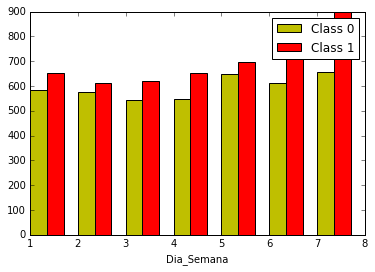
\includegraphics[width=7cm]{figs/dia_semana.png}
		\caption{Número de accidentes en los distintos días de la semana.}
		\label{fig:graf_tendencia}
	\end{center}
\end{figure}

\begin{figure}[htb!]
	\begin{center}
		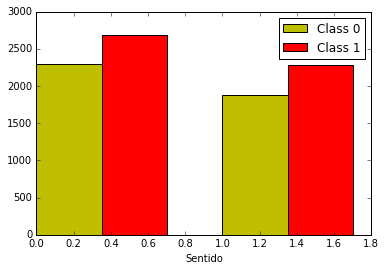
\includegraphics[width=6cm]{figs/hora.png}
		\caption{Número de accidentes dependiendo del sentido doble o no de la vías.}
		\label{fig:graf_no_tendencia}
	\end{center}
\end{figure}

También hemos comprobado la correlación lineal entre los distintos atributos utilizando el coeficiente de correlación de Pearson. Si dos atributos tienen una correlación muy alta, significa que existe una dependencia lineal entre ellos, y por lo tanto, comparten la misma información, por lo que podemos prescindir de uno de ellos. En este caso, hemos eliminado los atributos que presentaban una correlación superior al 75\%. De nuevo, hemos comparado los resultados antes y después de eliminar estos atributos para confirmar que no eliminamos nada que perjudique al rendimiento del modelo. \\

Al terminar con este proceso de análisis y extracción de características, hemos reducido los 83 atributos que tenían inicialmente los datos a 61. Aunque ha sido una reducción considerable, la dimensionalidad de los datos aún sigue siendo muy elevada. Por lo tanto, hemos probados los siguientes métodos de extracción de características para seleccionar las K mejores: \\

\begin{itemize}
	\item Principal Component Analysis (PCA)
	\item Truncated Singular Value Decomposition (SVD)
	\item Recursive Feature Extraction (RFE)
	\item Información mutua
	\item Mayor varianza \\
\end{itemize}

Para cada método y modelo hemos probado diferentes valores de K. Sin embargo, en todos los casos el resultado empeoraba al aplicar la extracción de características, consiguiendo mejores figuras de mérito al utilizar todos los atributos restantes. \\

\subsection{Selección del modelo}
Después de la extracción de características, el principal problema al que nos hemos enfrentado ha sido elegir el modelo más adecuado para este problema de clasificación. Los modelos considerados han sido los siguientes: \\

\begin{itemize}
	\item \textit{Multilayer Perceptron} - MLP
	\item \textit{Support Vector Machine} - SVM
	\item K-vecinos
	\item \textit{Probabilistic Neuronal Network} - PNN
	\item Regresor logístico
	\item Árboles de decisión \\
\end{itemize}

Sabiendo que el conjunto de test está desbalanceado, hemos considerado que la exactitud o \textit{accuracy} no era la mejor métrica para evaluar el rendimiento de los modelos, y hemos decidido utilizar la precisión o \textit{precision}. Inicialmente dividimos los datos en 10 grupos y usamos la función \textit{cross\_val\_score} proporcionada por la librería \emph{sk-learn}\cite{validacion_cruzada}, fijándonos en la media y la desviación estándar para comparar los resultados de los distintos modelos. Sin embargo, consideramos que el número de observaciones del que disponíamos era suficientemente grande, por lo que finalmente empleamos la división simple para su evaluación. De esta forma, además de agilizar el proceso de valoración de los modelos al probar distintas combinaciones de parámetros, la información que conseguíamos de cada realización era más detallada. Utilizamos la función \textit{classification\_report}, que basándose en la información de la matriz de confusión ofrece información sobre la precisión, sobre el \textit{recall} y el \textit{F1 score}, de cada clase y en media. \\

Para la evaluación de los modelos, el 80\% de los datos disponibles se han utilizado para entrenar el modelo (conjunto de entrenamiento) y el 20\% restante para evaluarlo (conjunto de validación). La separación de estos grupos se ha realizado de forma aleatoria y se ha supuesto que únicamente conocíamos los datos de entrenamiento, sin utilizar información procedente del conjunto de validación en ningún momento. \\

Después de definir estos conjuntos y el método empleado para la evaluación, empezamos a probar los distintos modelos anteriormente mencionados. Cada uno de estos modelos cuenta con unos parámetros distintos que hay que ajustar para que las predicciones de la máquina sean lo más precisas posibles. Para esto, seleccionamos los valores para los parámetros que consideramos más adecuados probando distintas combinaciones para cada modelo, entrenamos la máquina con el conjunto de entrenamiento y evaluamos su rendimiento utilizando el conjunto de validación. Con esta información, reajustamos los valores buscando siempre minimizar el error en el conjunto de validación, no en el de entrenamiento. Además, al haber más muestras de la clase 1 que de la clase 0 en el conjunto de test, nos centramos sobre todo en conseguir una precisión elevada en la clase 1. De esta forma asumimos costes asimétricos, dado que asignar a una observación la clase 0 cuando en realidad pertenecía a la clase 1 tenía un coste muy alto, mientras que, un falso positivo de la clase 1 no tenía tanto coste. Esto también tiene sentido desde el punto de vista de la situación real, dado que clasificar un accidente como leve cuando en verdad ha sido grave también supone un coste mayor que el error contrario, clasificarlo como grave cuando ha sido leve.  \\

Finalmente, cuando estamos satisfechos con la precisión obtenida con una determinada configuración del modelo, utilizamos el 100\% de los datos para entrenar la máquina, obtenemos las predicciones del conjunto de test y comprobamos los resultados. La motivación detrás de esto reside en que, teóricamente, así añadimos más datos al modelo al estar utilizando todas las observaciones disponibles, por lo que conseguimos que generalice mejor y se sobreajuste menos a los datos con los que se ha entrenado, obteniendo por lo tanto resultados mejores. \\


%%%%%%%%%% RESULTADOS %%%%%%%%%%
\section{Resultados}
\IEEEPARstart{E}n este capítulo hemos seleccionado los dos modelos que han dado mejores resultados, de todos los mencionados en el capítulo anterior. Para cada uno de ellos explicaremos la configuración de sus parámetros, las técnicas que hemos utilizado en su aprendizaje y expondremos los resultados que hemos obtenido con ellos.


\subsection{MLP}
Hay dos razones principales por las cuales hemos utilizado un MLP para resolver este problema de clasificación. En primer lugar, se trata de un estimador universal, por lo que eligiendo la arquitectura adecuada puede utilizarse para resolver cualquier problema, aunque encontrar esta arquitectura suele ser complicado dado que no existe ninguna regla que especifique como debe hacerse, si no que depende de cada situación concreta. La otra razón principal que nos llevó a utilizar este modelo es el amplio rango de parámetros modificables que proporciona la librería sklearn al utilizarlo. Esto proporciona una gran flexibilidad a la hora de entrenar el modelo, aunque también hace que sea necesario dedicarle más tiempo para encontrar los parámetros adecuados. Todos los parámetros que pueden seleccionarse para este modelo están descritos en \cite{mlp}. \\

Para resolver este problema hemos probado múltiples combinaciones de redes neuronales, variando los valores de distintos parámetros. Los parámetros principales que hemos ajustado han sido los siguientes: \\

\begin{itemize}
	\item El número de neuronas de cada capa oculta y el número de capas ocultas.  \\
	\item La función de activación, eligiendo entre la función identidad, la función sigmoide, la tangente hiperbólica y un rectificador linear uniforme (RLU). \\
	\item El valor inicial de la tasa de aprendizaje.  \\
	\item Hemos probado manteniendo la tasa de aprendizaje fija, tasa de aprendizaje adaptativa o con escalado inverso.  \\
	\item La tolerancia, que es el valor utilizado para detectar si el algoritmo de optimización ha alcanzado un mínimo. Si la diferencia entre el error de la iteración anterior y la iteración actual no supera el valor de la tolerancia, el algoritmo se detendrá.  \\
	\item Hemos probado con y sin la técnica de \textit{early stopping}. Con esta técnica, el algoritmo utiliza un porcentaje del conjunto de entrenamiento como conjunto de validación para comprobar cuando el error en este conjunto alcanza un mínimo y dejar de iterar. Este valor también lo hemos ajustado.   \\
	\item El número máximo de iteraciones (importante cuando no utilizamos \textit{early stopping}).  \\
	\item Distintos algoritmos para minimizar el error como lbfgs, descenso por gradiente estocástico y Adam.  \\
	\item El término de regularización \textit{alpha}.  \\
\end{itemize}

En la tabla \ref{tabla:tabla_mlp} se muestran los modelos que mejores resultados nos han dado basándonos en redes neuronales, indicando los parámetros que varían entre ellos. Además de los valores indicados en dicha tabla, todos ellos utilizan como función de activación un RLU, el método Adam como algoritmo para minimizar el error, un valor de 1·10\textsuperscript{-12} para la tolerancia, 1·10\textsuperscript{-4} para alfa y una tasa de aprendizaje inicial con un valor de 0.1. Además, el conjunto de validación para el \textit{early stopping} es el 20\% del conjunto de entrenamiento. En esta tabla observamos también que hay dos combinaciones que han obtenido la puntuación más alta sobre el conjunto de test, un MLP con 3 capas ocultas y 5 neuronas por cada capa, y otro con 3 capas de 100 neuronas cada una.


\begin{table}[htb!]
	\begin{center}
		\caption{Resultados de distintos modelos del MLP}
		\begin{tabular}{| m{2.1cm} | m{1cm} | m{1cm} | m{1cm} | m{1.2cm} |}
			\hline
			Modelo & Precisión Clase 0 & Precisión Clase 1 & Precisión Media & Puntuación Test   \\ \hline
			capa oculta: (50,3) tasa de aprendizaje: constante & 0.37                & 0.86                & 0.74              & 0.765  \\ \hline
			capa oculta: (100,3), tasa de aprendizaje: constante & 0.17                & 0.95               & 0.87             & 0.765  \\ \hline
			capa oculta: (40,3), tasa de aprendizaje: constante & 0.8 & 0.44 & 0.68 & 0.62 \\ \hline
			capa oculta: (100,1), tasa de aprendizaje: contante & 0.22 & 0.92 & 0.81 & 0.75    \\ \hline
			capa oculta: (100,3), tasa de aprendizaje: adaptativa & 0.22 & 0.92 & 0.81 & 0.75 \\ \hline
			
		\end{tabular}
		
		\label{tabla:tabla_mlp}
	\end{center}
\end{table}


\subsection{SVM}

Aunque SVM no fue el primer modelo que consideramos, ha resultado ser el que mejor resultados nos ha dado. La principal razón por la que nos inclinamos a utilizarlo fue que, aunque no podemos representar los resultados por trabajar con dimensiones demasiado altas, resulta más intuitivo pensar que está pasando al modificar los parámetros. La idea básica del Modelo de Máquinas de Vectores Soporte (SVM) es encontrar el hiperplano óptimo que separe linealmente los datos. Sin embargo, como este conjunto de datos no es linealmente separable hemos tenido que utilizar el método del kernel, aplicando a los datos una transformación trasladándolos a otro espacio de representación en el que sí son linealmente separables, de forma que se consigue una separación no lineal en el espacio original. La función responsable de esta transformación es uno de los parámetros que hemos variado para encontrar la mejor solución al problema. De nuevo, hemos utilizado la librería \textit{sklearn}, y todos los parámetros que pueden seleccionarse para este modelo están descritos en \cite{svm}. \\

Al igual que en el caso del MLP, para encontrar el mejor modelo posible hemos probado distintas combinaciones de SVMs, variando el valor de distintos parámetros y comprobando si mejoraba o no el rendimiento. Los principales parámetros que hemos ajustado han sido: \\

\begin{itemize}
	\item La función kernel a utilizar para la transformación del espacio. Esto es especialmente importante dado que no se pueden conseguir buenos resultados en una SVM si la transformación no es la adecuada. Las principales funciones que hemos barajado han sido: polinómica variando el grado, rbf (función de base radial) y sigmoide, siendo la función polinómica la que mejores resultados ha conseguido. \\
	\item El coste con el que se penalizará los datos clasificados de forma errónea dentro de los vectores soporte. Este parámetro también ha sido especialmente importante debido a la gran cantidad de ruido existente en los datos. \\
	\item El grado en el caso de estar utilizando una funció polinómica. \\
	\item El valor de gamma, que es el coeficiente del kernel para las funciones rbf, polinómicas y sigmoides. Cuando este parámetro se establece a \textit{auto}, su valor será 1/número\_características. \\
\end{itemize}

Tras probar distintas combinaciones de estos parámetros, la tabla \ref{tabla:tabla_svm} muestra las combinaciones que mejores resultados han dado. En este caso se puede observar que, aunque la mayoría de los resultados son bastante próximos, la combinación que ha obtenido mejores resultados en el conjunto de test ha sido la primera, utilizando un kernel polinómico de grado 3, un coste de 0.035 y un valor de gamma de 1/61.

\begin{table}[htb!]
	\begin{center}
		\caption{Resultados de distintos modelos de SVM}
		\begin{tabular}{| m{2.1cm} | m{1cm} | m{1cm} | m{1cm} | m{1.2cm} |}
			\hline
			Modelo & Precisión Clase 0 & Precisión Clase 1 & Precisión Media & Puntuación Test   \\ \hline
			kernel: polinómica, grado: 3, C: 0.035, gamma: "auto" & 0.14                & 0.97                & 0.9              & 0.78  \\ \hline
			kernel: polinómica, grado: 3, C: 0.045, gamma: "auto" & 0.17                & 0.94               & 0.86             & 0.77  \\ \hline
			kernel: polinómica, grado: 3, C: 0.025, gamma: "auto" & 0.12 & 0.96 & 0.9 & 0.765 \\ \hline
			kernel: polinómica, grado: 5, C: 0.02, gamma: "auto" & 0.11 & 0.96 & 0.91 & 0.76    \\ \hline
			kernel: rbf, gamma: 0.12, C: 0.035 & 0.15 & 0.92 & 0.84 & 0.765 \\ \hline
			
		\end{tabular}
		
		\label{tabla:tabla_svm}
	\end{center}
\end{table}


%%%%%%%%%% CONCLUSIONES %%%%%%%%%%
\section{Conclusiones}
Tras el análisis de los diferentes modelos planteados, los mejores resultados los han ofrecido los modelos correspondientes al MLP y SVM. Utilizando estos dos modelos con sus diferentes configuraciones, explicadas en el apartado anterior, si comparamos las tablas \ref{tabla:tabla_mlp} y \ref{tabla:tabla_svm} podemos observar que han tenido unos resultados similares. En el caso del MLP hay dos modelos que nos han reportado un acierto del 76.5\% sobre el conjunto de test. Con el primero, formado por 3 capas ocultas y 50 neuronas por capa hemos conseguido una precisión del 37\% en la clase 0, del 86\% en la clase 1 y de del 74\% en media. El segundo, constituido por 3 capas ocultas de 100 neuronas cada una ha conseguido una precisión del 17\% en la clase 0, del 95\% en la clase 1 y del 87\% en media. Así mismo, el modelo SVM formado por una función de kernel polinómica de grado 3 y un coste de penalización de 0.035 ha conseguido una precisión en la clase 0 del 14\%, del 97\% en la clase 1 y una precisión media del 90\%. Además, ha reportado un acierto del 78\% en el conjunto de test. Por lo tanto, el modelo que mejores resultados ha dado ha sido el SVM, aunque el MLP no se sitúa muy lejos, sólo un 1.5\% por debajo.\\

Cómo ya habíamos explicado en la introducción, este problema forma parte de un concurso creado por la Universidad Rey Juan Carlos, y hemos presentado el modelo que nos ha aportado un mejor resultado en el conjunto de test. Este modelo ha sido la primera combinación de SVM que aparece en la tabla \ref{tabla:tabla_svm}. Una vez terminada la competición y publicada la tabla de clasificación, el modelo presentado nos ha colocado en el segundo puesto de la competición, entre más de 6 equipos participantes.\\

Para concluir, uno de los aspectos principales a destacar de este documento, es que prueba los conocimientos adquiridos en la asignatura. Consideramos que hemos plasmado todo lo aprendido, tanto desde el punto de vista de análisis y tratamiento de datos y extracción de características, como desde el estudio y conocimiento de los distintos modelos de clasificación que hemos visto. Además, todo el código se ha escrito en Python, mostrando que comprendemos y conocemos las librerías para realizar tareas de \textit{Machine Learning} en este lenguaje.

\begin{thebibliography}{1}

\bibitem{analisis_datos}
Figuera, C., Lillo, J. M., Mora-Jimenez, I., Rojo-Álvarez, J. L., \& Caamaño, A. J. (2011, October). \emph{Multivariate spatial clustering of traffic accidents for local profiling of risk factors.} In Intelligent Transportation Systems (ITSC), 2011 14th International IEEE Conference on (pp. 740-745). IEEE.

\bibitem{extraccion_datos}
Mitchell, T. M. (2006). \emph{The discipline of machine learning (Vol. 9).} Carnegie Mellon University, School of Computer Science, Machine Learning Department.

\bibitem{alta_dimensionalidad}
Domingos, P. (2012). \emph{A few useful things to know about machine learning.} Communications of the ACM, 55(10), 78-87.

\bibitem{validacion_cruzada}
\emph{Cross-validation: evaluating estimator performance} http://scikit-learn.org/stable/modules/cross\_validation.html

\bibitem{mlp}
\emph{MLP Classifier in scikit-lear.}
http://scikit-learn.org/stable/modules/generated/sklearn.neural\_network.MLPClassifier.html

\bibitem{svm}
\emph{Support Vector Classification}
http://scikit-learn.org/stable/modules/generated/sklearn.svm.SVC.html

\end{thebibliography}
\end{document}


